
Spurious signals may occur from statistical fluctuations. Therefore, in this section, we test toy datasets to check if there are signal like structures. The toy datasets are signal-free datasets (no signals injected), and generated total of 1000 samples. Each sample (toy dataset) is fitted 12 times, each time with different signal shapes (we have total of 12 signals). Each fit will estimate a coefficient. 

Figure~\ref{fig:spurious_test} shows distributions of 4 example coefficients ($d_u^{XZ}\equiv d_{0}$, $d_u^{YZ} \equiv d_{1}$, $d_u^{XX-YY} \equiv d_{2}$ and $d_u^{XY} \equiv d_{3}$) estimated from 1000 toy datasets. From each plot we can see that mean of each distribution is very close to zero. The Figure~\ref{fig:spurious_test_summary} shows mean and standard deviation of the distributions shown in Figure~\ref{fig:spurious_test}, expanded to all 12 coefficients.



\begin{figure}[!htb]
	\centering
	\subfloat{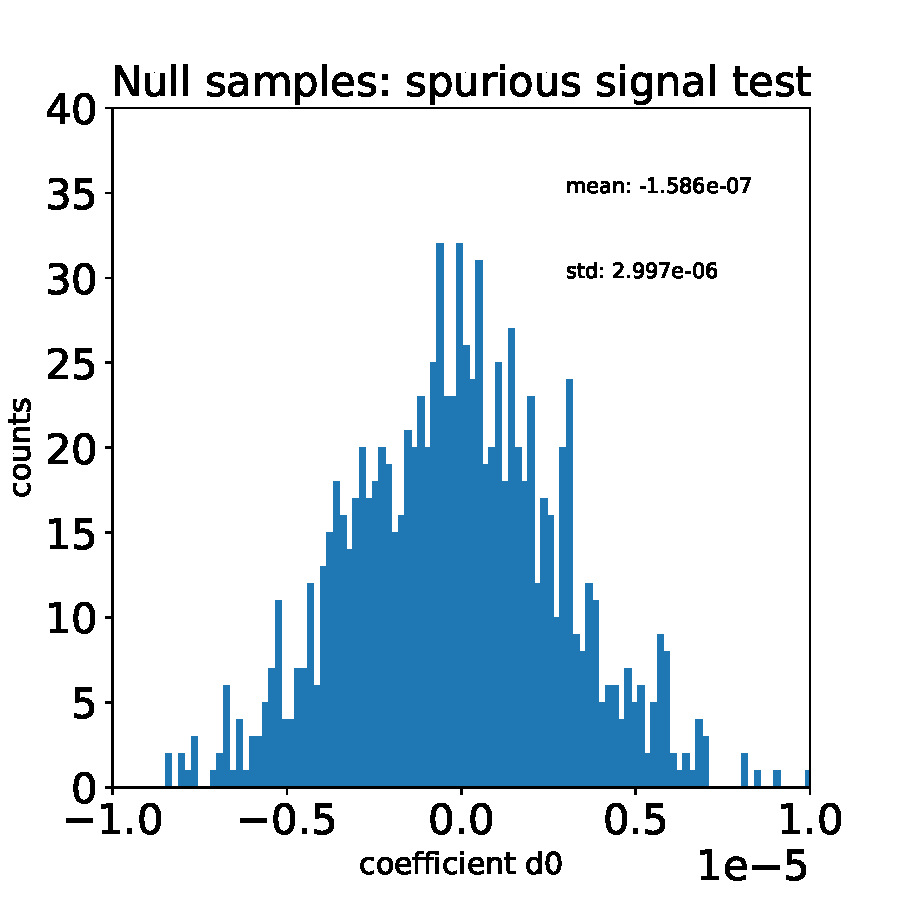
\includegraphics[width=0.48\textwidth]{figs/spurious_test/Null_spurious_test_d0}}
	\subfloat{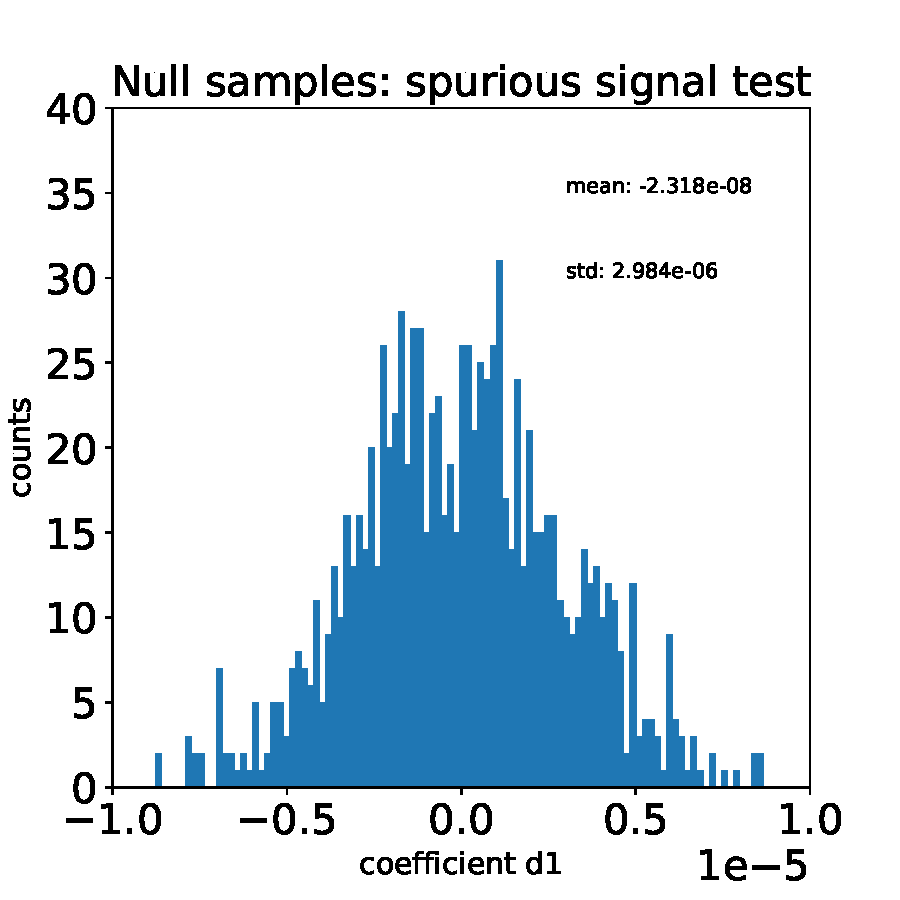
\includegraphics[width=0.48\textwidth]{figs/spurious_test/Null_spurious_test_d1}}\\
	\subfloat{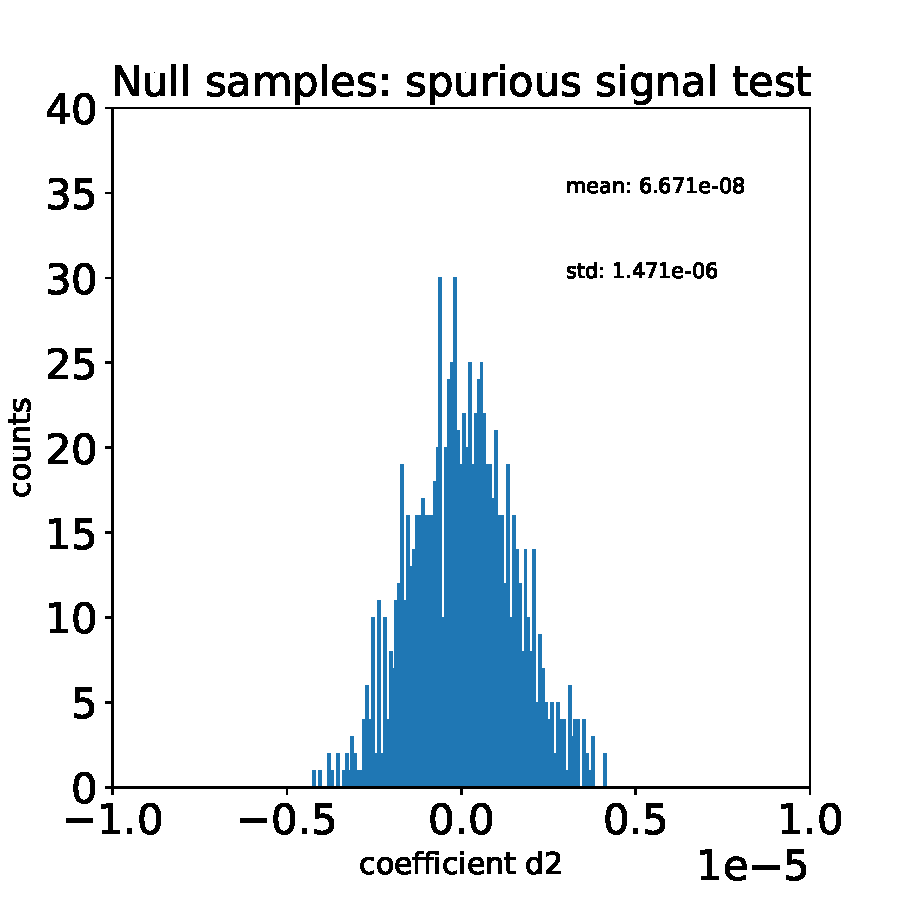
\includegraphics[width=0.48\textwidth]{figs/spurious_test/Null_spurious_test_d2}}
	\subfloat{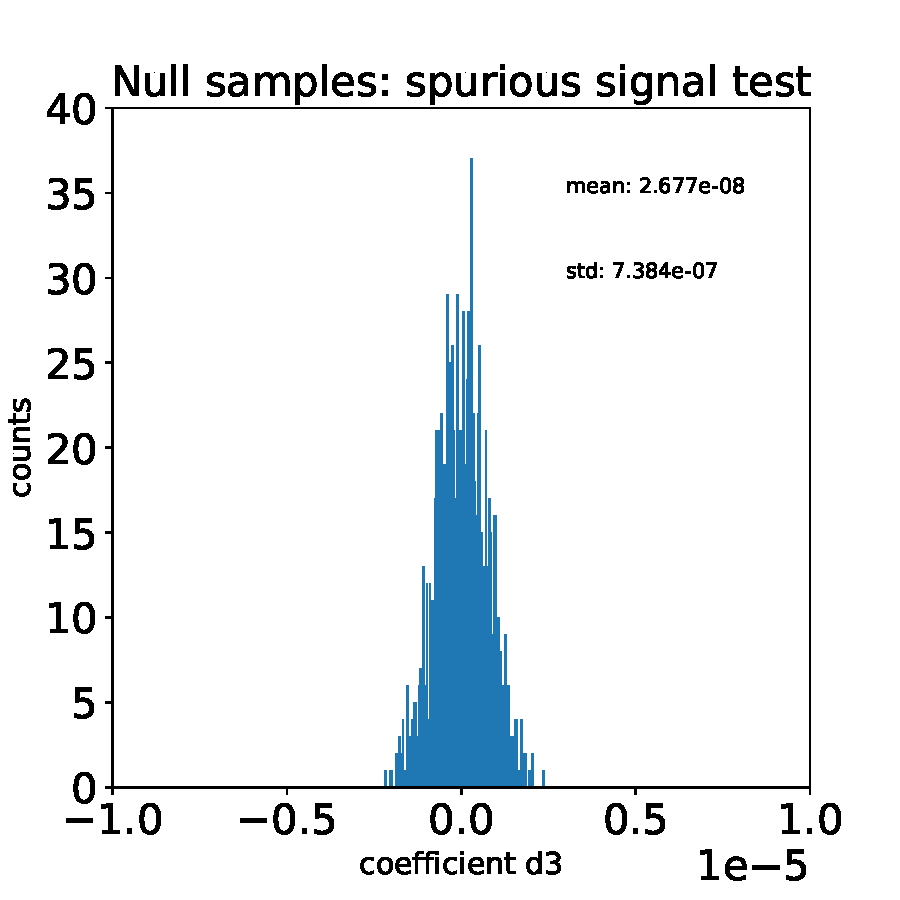
\includegraphics[width=0.48\textwidth]{figs/spurious_test/Null_spurious_test_d3}}
    \caption{Results of spurious signal tests on 1000 signal-free toy datasets. Top left is a distribution of estimated $d_{0}$ parameters, top right is $d_{1}$ parameters, bottom left is $d_{2}$ parameters and bottom right is $d_{3}$ parameters.}
	\label{fig:spurious_test}
\end{figure}


\begin{figure}[!htb]
	\centering
	\subfloat{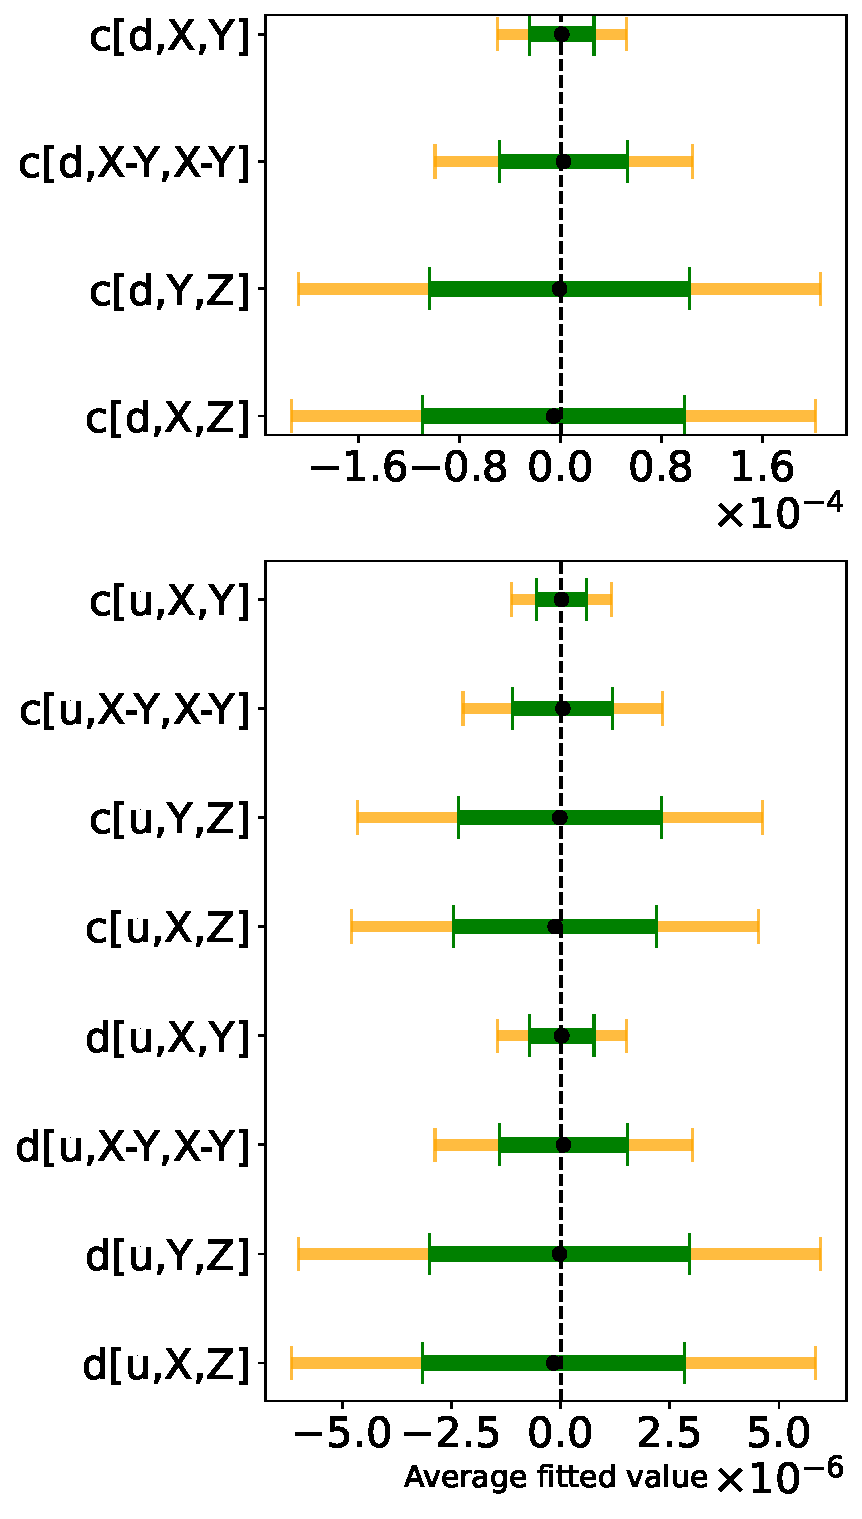
\includegraphics[width=0.48\textwidth]{figs/spurious_test/Null_SigFit_summary_1000samples}}

     \caption{Summary of spurious signal tests on 1000 signal-free toy datasets. Black dot is a numpy mean of corresponding distributions
       in the Figure~\ref{fig:spurious_test}, the green and orange bands are one and two standard diviations calculated with the numpy function. }
	\label{fig:spurious_test_summary}
\end{figure}

